
\documentclass[12pt]{article}
\usepackage{graphicx}
\usepackage{amsmath}
\usepackage{mathtools}
\usepackage{gensymb}

\newcommand{\mydet}[1]{\ensuremath{\begin{vmatrix}#1\end{vmatrix}}}
\providecommand{\sbrak}[1]{\ensuremath{{}\left[#1\right]}}	
\providecommand{\brak}[1]{\ensuremath{\left(#1\right)}}
\providecommand{\norm}[1]{\left\lVert#1\right\rVert}
\providecommand{\abs}[1]{\left\vert#1\right\vert}
\newcommand{\solution}{\noindent \textbf{Solution: }}
\newcommand{\myvec}[1]{\ensuremath{\begin{pmatrix}#1\end{pmatrix}}}
\let\vec\mathbf

\begin{document}
\begin{center}
\textbf\large{CONIC SECTIONS}

\end{center}
\section*{Excercise 8.2}
Q2.Find the area bounded by the curves $\brak{x-1}^2 + y^2 = 1 \text{ and } x^2+y^2=1$.

\solution
The general equation of a conic is given as
\begin{align}
	\label{eq:eq1}
	g\brak{\vec{x}} = \vec{x}^\top \vec{V}\vec{x}+2\vec{u}^\top \vec{x}+f=0
\end{align}
The first curve equation can be rearranged as
\begin{align}
	\label{eq:eq2}
	x^2+y^2-2x=0
\end{align}
Comparing \eqref{eq:eq1} and \eqref{eq:eq2} we get
\begin{align}
	\vec{V} &= \myvec{1&0\\0&1}\\
	\vec{u} &= \myvec{-1\\0}\\
	f &= 0
\end{align}
The second curve equation can be rearranged as
\begin{align}
	\label{eq:eq3}
	x^2+y^2-1=0
\end{align}
Comparing \eqref{eq:eq1} and \eqref{eq:eq3} we get
\begin{align}
	\vec{V} &= \myvec{1&0\\0&1}\\
	\vec{u} &= \myvec{0\\0}\\
	f &= -1
\end{align}
The intersection of conics is obtained as
\begin{align}
	\vec{x}^\top\brak{\vec{V}_1+\mu\vec{V}_2}\vec{x}+2\brak{\vec{u}_1+\mu\vec{u}_2}^\top\vec{x}+\brak{f_1+\mu f_2}=0
\end{align}
The locus of the intersection is a pair of straight lines if
\begin{align}
	\mydet{\vec{V}_1+\mu\vec{V}_2 & \vec{u}_1+\mu\vec{u}_2 \\ \brak{\vec{u}_1+\mu\vec{u}_2} & f_1+\mu f_2} = 0
\end{align}
On substituting values we get
\begin{align}
	\mydet{1+\mu & 0 & -1 \\ 0 & 1+\mu & 0 \\ -1 & 0 & -\mu} = 0
\end{align}
solving the determinant we get
\begin{align}
	\mu^3+2\mu^2+2\mu+1&=0\\
	\implies \mu &= -1
\end{align}
Thus, the parametrs for straight line cann be expressed as
\begin{align}
	\vec{V} &= \vec{V}_1+\mu\vec{V}_2 = \myvec{0&0\\0&0}\\
	\vec{u} &= \vec{u}_1+\mu\vec{u}_2 = \myvec{-1\\0}\\
	f &= 1
\end{align}
Substituting these values we get
\begin{align}
	\vec{x}^\top\myvec{0&0\\0&0}\vec{x} + 2\myvec{-1&0}\vec{x} + 1 &= 0\\
	\myvec{-2&0}\vec{x} &= -1 
\end{align}
Therefore
\begin{align}
	\vec{m} = \myvec{0\\1} \text{ and } \vec{h} = \myvec{\frac{1}{2}\\0}
\end{align}
Now intersection of line with a conic is given by
\begin{align}
	\vec{x}_i=\vec{h}+\mu_i\vec{m}
\end{align}
where
\begin{align}
	\label{eq:eq4}
	\mu_i=\frac{1}{\vec{m}^\top\vec{V}\vec{m}}\brak{-\vec{m}^\top\brak{\vec{V}\vec{h}+\vec{u}}\pm\sqrt{\sbrak{\vec{m}^\top\brak{\vec{V}\vec{h}+\vec{u}}}^2-g\brak{\vec{h}}\brak{\vec{m}^\top\vec{V}\vec{m}}}}
\end{align}
Now
\begin{align}
	g\brak{\vec{h}}&=\myvec{\frac{1}{2}&0}\myvec{1&0\\0&1}\myvec{\frac{1}{2}\\0}+2\myvec{0&0}\myvec{\frac{1}{2}\\0}-1\\
	&= -\frac{3}{4}\\
	\vec{m}^\top\vec{V}\vec{m} &= \myvec{0&1}\myvec{1&0\\0&1}\myvec{0\\1} = 1\\
	\vec{m}^\top\brak{\vec{V}\vec{h}+\vec{u}} &= 0
\end{align}
substituting in \eqref{eq:eq4} we get
\begin{align}
	\mu_i = \pm\frac{\sqrt{3}}{2}
\end{align}
Hence the point of intersection are
\begin{align}
	\vec{a}_0 = \myvec{\frac{1}{2}\\\frac{\sqrt{3}}{2}}, \vec{a}_2 = \myvec{\frac{1}{2}\\-\frac{\sqrt{3}}{2}}
\end{align}
The desired area of region is given as
\begin{align}
	&=2\brak{\int_{0}^{\frac{1}{2}} \sqrt{1-\brak{x-1}^2}dx + \int_{\frac{1}{2}}^{1} \sqrt{1-x^2}dx}\\
	\begin{split}
		&{}=2\sbrak{\frac{1}{2}\brak{x-1}\sqrt{1-\brak{x-1}^2}+\frac{1}{2}\sin^{-1}\brak{x-1}}_{0}^{\frac{1}{2}}\\
		& +2\sbrak{\frac{x}{2}\sqrt{1-x^2}+\frac{1}{2}\sin^{-1}x}_{\frac{1}{2}}^{1}
	\end{split}\\
	&= \frac{2\pi}{3}-\frac{\sqrt{3}}{2}
\end{align}
See figure \ref{fig:Fig1}
\begin{figure}[!h]
	\begin{center} 
	    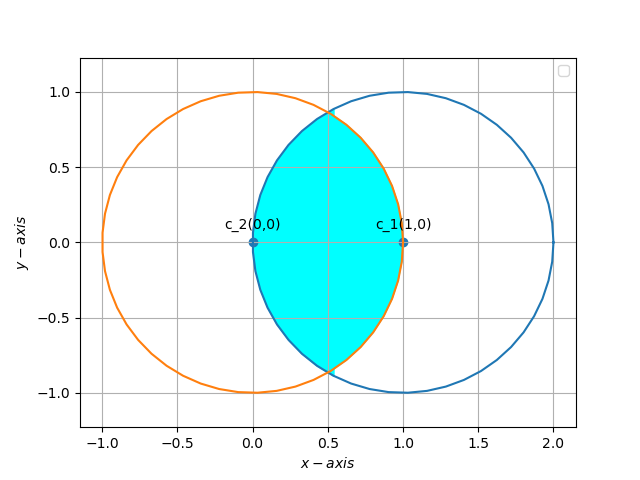
\includegraphics[width=\columnwidth]{figs/inter1}
	\end{center}
\caption{}
\label{fig:Fig1}
\end{figure}
\end{document}


















